

SN cosmology is systematics-limited. Increasing the statistics in the
Hubble diagram must be coupled with (1) advances in the measurement of
the SN distances (i.e.  a control at the per-mil level of the
photometry and survey flux calibration, and possibly a 3-parameter SN
standardization technique) (2) a better control of the SN
astrophysical environment and its potential impacts on the SN
light curves and distances (local host properties, absorption) (3) a
better control of the SN diversity (SN~Ia sub-populations, population
drift with redshift) (4) a precise determination of the survey
selection function (SN identification, residual contamination by
non-SN~Ia's as a function of redshift).

Access to spectroscopy will not scale with the large amount of SNe
LSST will deliver.  About 10\% of LSST SNe will benefit from a live
spectrum.  Securing spectroscopic host redshifts for the full LSST
sample using the fiber spectrographs available in the southern
hemisphere is challenging -- although doable.  As a consequence, all
the studies listed above, in particular SN~Ia identification and the
standardization of SN luminosity distances will rely on the supernova
light curves only.  Obtaining high quality SN light curves is
therefore a key design point of the SN survey.  The average quality of
the SN light curves depends exclusively on the observing strategy.

Furthermore, spectroscopic time being scarse, we cannot afford to
waste it.  This means that all transients identified
spectroscopically, around peak luminosity, as SNe~Ia, {\em must}
eventually have light curves of sufficient quality to end up in the
Hubble diagram.  This puts another requirement on the regularity and
predictability of the observing strategy.

Since light curve quality is at the core of the design of the LSST SN
survey, we propose to adopt as our main metric, the size and redshift
extent of the subset of well sampled SNe~Ia.  We define in the next
section what we mean by ``well-sampled''.


Four key facets of observing strategy that have an impact on the number and on the quality of well-measured supernovae may be identified: {\it a regular cadence} (typical values: three to four days) is important to get well-sampled light curves ; minimal inter-night gaps are mandatory to keep a high detection efficiency of the supernovae; the {\it season length} has an impact on the total number of supernovae that may be collected ; 170 to 180 days are values of interest for supernova science; {\it depth} quantified by m5, the five-sigma depth, which is the magnitude corresponding to a flux with a signal-to-noise ratio (SNR) equal to 5. Since only light curve points of well-measured supernovae with SNR $>$5 are considered, m5 has an impact on the redshift limit of observation (photostatistic limit); {\it spatial coverage and uniformity} which has an impact both on the wide and on the deep surveys; it may be interesting to observe deep fields evenly distributed in Ra (and Galactic/Ecliptic planes avoided) so as to search for anisotropies using individual Hubble diagrams.


\subsection{Requirements on SN sampling}
\label{sec:sn_sampling_requirements}

Light curves are the essential ingredient to (1) measure standardized
luminosity distances and (2) photometrically identify SNe~Ia from
their full light curve. This drives a series of requirements which we
summarize below.

\begin{enumerate}

\item each SN must have good quality measurements in at least three
  bands. We need two bands, covering the restframe $B$ and $V$ region,
  to constrain the restframe color of the SN. We need to provision an
  additional band (redder than restframe $V$), to enable next
  generation standardization techniques, that will likely rely on two
  restframe colors.

\item the follow-up of each supernova must be good enough in the
  observer-frame bands that correspond to the $B$- and $V$-restframe
  spectrum ($3800 \angstrom < \lambda < 7000 \angstrom$).  At
  high-redshift, in particular, one should avoid relying on the $UV$
  restframe region to derive a distance, given the high intrinsic
  dispersion of SN~Ia at those wavelengths.
  
\item we require the light curve shape to be well sampled in the
  (restframe) phase interval $[-10;+30]$ days, with at least five
  visits before peak (each of those visits in any of the eligible
  band), and ten visits after peak.  To obtain this in the lower
  redshift region of the Hubble diagram, one requires an
  observer-frame cadence of 4 days.  At higher redshifts redshifts
  (DDF fields), this requirement may be slightly relaxed. However,
  since we are going to rely almost exclusively on photometric
  identification, it is essential to secure a tight sampling of the SN
  color evolution at all redshift.
  
\item we require that the photon noise contribution to the distance
  measurement is subdominant w.r.t. the intrinsic dispersion of the
  SNe (after standardization).  There are several ways to quantify
  this.  With today's standardization techniques, the SN standardized
  distance modulus is:
  \begin{equation}
    \mu = m^\star_B + \alpha X_1 - \beta C - \cal{M}
  \end{equation}
  where $m^\star_B$ is the peak brightness in restframe $B$, $X_1$
  characterize the lightcurve width, and $C$ is an estimate of the
  restframe color $B-V$. $\alpha$, $\beta$ and $\cal{M}$ are global
  parameters, fit along with the cosmology. If the light curve is
  correctly sampled (see point above), the propagation of the
  measurement uncertainties affecting $m^\star_B$, $X_1$ and $C$ is
  dominated by the contribution of $\sigma_C$. (since $\beta \sim
  3$). In practice, requiring $\sigma C < 0.04$ ensures that $\sigma
  \mu < 0.1$, below the intrinsic dipersion in the Hubble diagram,
  after standardization.
\end{enumerate}

This last requirement may be re-expressed as a requirement on the
signal-to-noise on the light-curve amplitude in each band. Indeed, if
we fit a light curve model $L(t) = A \times \ell(t)$ one can show
that:
\begin{equation}
\mathrm{SNR_{band}} = \sum_{i} 5 \times (f^{-2}_{i|5} L_i^2)^{1/2}\label{eqn:snr}
\end{equation} 
where $5-\sigma$ is the limiting flux of each visit $f_{i|5}$.  This
metrics is simpler in the sense that it does not require to use a SN
light curve fitter. One just need lightcurve templates and the
limiting magnitudes of each visit -- given in the cadence
databases. In practice, using $SNR_g > 30, SNR_r > 40, SNR_i > 30$
(for $z<0.3$), and $SNR_r > 40$, $SNR_i > 30$ and $SNR_z > 20$ for
$z>0.3$ allows to fulfill the requirement on color resolution above.


\subsection{SN samples}

The SN sample usable for cosmology can be defined from the light curve
requirements listed in the previous section. The key quantity is the
redshift limit, $z_{lim}$, beyond which one starts loosing events
because of poor sampling.  This ``redshift-limit'' is not a
detectability limit.  It is the redshift value beyond which we start
losing a fraction of the events, because their photometric follow-up
does not match the requirements listed in the previous section.

The definition of the redshift limit depends on the intrinsic
luminosity of the supernova considered.  SN~Ia luminosities can be
parametrized using two parameters, e.g. lightcurve width ($X_1$) and
SN restframe B-V color at peak ($C$).  As shown on figure
\ref{fig:jla_X1_C}, the SN distribution in this parameter space is
compact and more than 95\% of the statistics can be enclosed in a
tight ellipse. 

\begin{figure}
  \begin{center}
    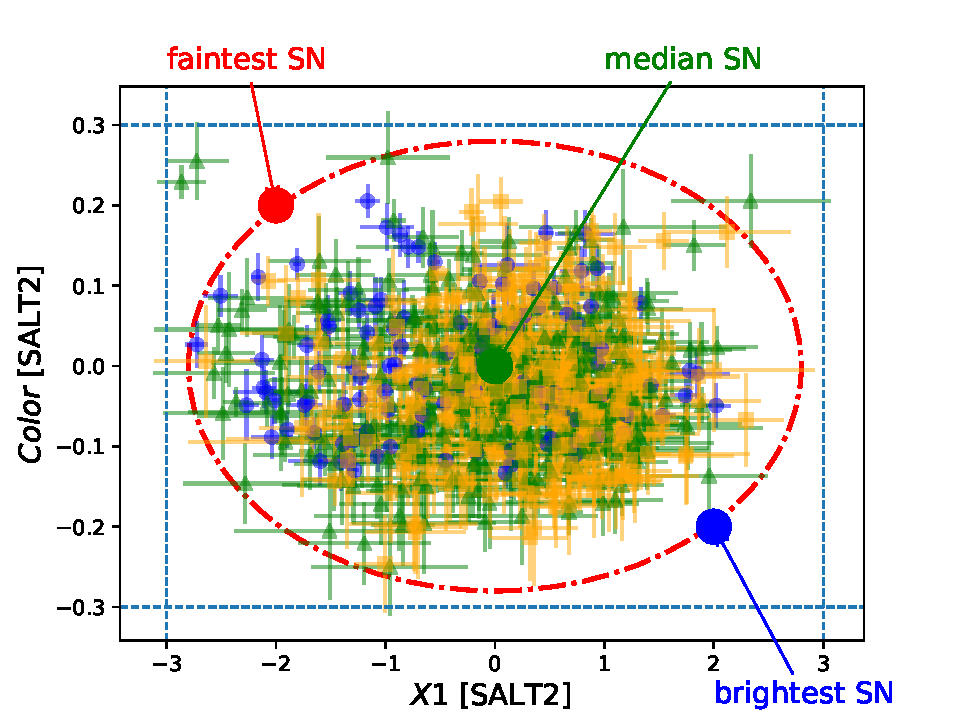
\includegraphics[width=0.6\textwidth]{key_design/sn_parameter_space.pdf}
    \caption{JLA supernovae the $(X_1,Color)$ parameter space --
      (blue: nearby, green: SDSS, orange: SNLS).  The large dots
      indicate the position of the faint, median and bright fiducial
      SNe used for the cadence analyses.}
    \label{fig:jla_X1_C}
  \end{center}
\end{figure}

On the same figure, we have represented three fiducial SNe of
particular interest: the red dot represents the faintest SN in this
region of the parameter space $(X_1=-2, C=0.2)$, the green dot and
blue dots show the average $(X_1=0, C=0)$ and brightest SN $(X_1=2,
C=-0.2)$ respectively.

We can define the redshift limit \zfaint as the limit beyond which the
faintest fiducal SN no longer passes the light curve requirements. By
doing this, we ensure that all SNe that live in the fiducial $(X_1,C)$
parameter space and are below \zfaint do pass our light curve
requirements.  \zfaint defines a {\em redshift-limited sample} whose
selection function does not depend on the SN properties.

We can also define a similar limit, using the median supernova,
instead of the faint one.  This defines a SN sample whose upper
redshift bins are affected by a selection bias, which must be
determined using a simulation -- which itself depends on our knowledge
of the SN luminosity distribution at those redshifts.  The uncertainty
affecting the determination of the selection function generally limits
the usefulness of the redshift bins affected by a selection bias.
Since the selection function is generally symmetric around its 50\%
point, the size of the sample limited by \zmed gives a good
approximation of the total number of LSST SNe that will have precise
distances.


\subsection{Metrics}
\label{sec:metrics}
We propose to use as our primary metrics the size and depth of the
subset of well sampled SNe.  More precisely, we estimate, for each
cadence, the following quantities:

\begin{itemize}
\item the sample redshift limit, \zfaint defined above, and the number
  of well sampled supernovae below the redshift limit \nsnfaint
\item the redshift \zmed at which the median supernova defined above
  no longer passes the signal-to-noise requirements, and the number of
  well-sampled supernovae below this redshift, \nsnmed.  
\end{itemize}
The former give an assessment of the size and depth of the redshift
limited sample, i.e. the sample of supernovae usable for cosmology,
and whose selection function is extremely easy to determine.  The
latter gives an assessment of the size and depth of the sample of SNe
that will have precise distances.
